% Relatório do Trabalho Prático — Sistemas Distribuídos II (Unimontes)
% Compilar dentro de docs/relatorio:   latexmk -pdf relatorio.tex
% As figuras de evidência são lidas diretamente de ../../evidencias/.
\documentclass[11pt,a4paper]{article}

\usepackage[T1]{fontenc}
\usepackage[utf8]{inputenc}
\usepackage[brazil]{babel}
\usepackage{lmodern}
\usepackage{microtype}
\usepackage[a4paper,margin=2.5cm]{geometry}
\usepackage{graphicx}
\usepackage{float}
\usepackage{booktabs}
\usepackage{tabularx}
\usepackage{longtable}
\usepackage{array}
\usepackage{enumitem}
\usepackage[table]{xcolor}
\usepackage{listings}
\usepackage{caption}
\usepackage{fancyhdr}
\usepackage{tikz}
\usetikzlibrary{arrows.meta,positioning,shapes.geometric,fit,calc,backgrounds}
\usepackage[hidelinks]{hyperref}

\graphicspath{{figuras/}{../../evidencias/}}

% ------------------------------------------------------------------ dados
\newcommand{\disciplina}{Sistemas Distribuídos II}
\newcommand{\professor}{Prof. Marcel Veloso Campos}
\newcommand{\titulo}{Chat distribuído com sockets, threads, TLS e bot com LLM}
% Preencher os sobrenomes de Bruna e Fellipe:
\newcommand{\integrantes}{Pedro Henrique Esteves Sarmento \\ Bruna \\ Fellipe}
\newcommand{\repositorio}{\url{https://github.com/PedroSarmentoo/ProjetoFinalSD2}}

% ------------------------------------------------------------------ estilo
\definecolor{azul}{HTML}{1F5FA8}
\definecolor{cinza}{HTML}{5A6270}
\definecolor{fundo}{HTML}{F4F6F9}
\definecolor{verde}{HTML}{2E7D32}
\definecolor{vermelho}{HTML}{C62828}
\definecolor{roxo}{HTML}{6A3FB0}

\setlist{itemsep=2pt,topsep=4pt}
\captionsetup{font=small,labelfont=bf,format=hang}
\setlength{\parskip}{4pt}
\renewcommand{\arraystretch}{1.18}

\pagestyle{fancy}
\fancyhf{}
\fancyhead[L]{\small\color{cinza}\disciplina}
\fancyhead[R]{\small\color{cinza}\titulo}
\fancyfoot[C]{\small\thepage}
\renewcommand{\headrulewidth}{0.3pt}

\lstset{
  basicstyle=\ttfamily\footnotesize,
  backgroundcolor=\color{fundo},
  frame=single, rulecolor=\color{black!15},
  breaklines=true, breakatwhitespace=false,
  columns=fullflexible, keepspaces=true,
  showstringspaces=false,
  xleftmargin=4pt, xrightmargin=4pt, aboveskip=6pt, belowskip=6pt,
  literate={á}{{\'a}}1 {à}{{\`a}}1 {ã}{{\~a}}1 {â}{{\^a}}1 {é}{{\'e}}1 {ê}{{\^e}}1
           {í}{{\'i}}1 {ó}{{\'o}}1 {õ}{{\~o}}1 {ô}{{\^o}}1 {ú}{{\'u}}1 {ç}{{\c c}}1
           {Á}{{\'A}}1 {É}{{\'E}}1 {Ç}{{\c C}}1 {→}{{$\rightarrow$}}1 {—}{{---}}1
           {…}{{\ldots}}1 {·}{{$\cdot$}}1
}
\lstdefinestyle{py}{language=Python, keywordstyle=\color{azul}\bfseries,
  commentstyle=\color{cinza}\itshape, stringstyle=\color{verde}}

\newcommand{\cod}[1]{\texttt{#1}}
\newcommand{\tipo}[1]{\texttt{\textbf{#1}}}

\begin{document}

% ================================================================== CAPA
\begin{titlepage}
\centering
{\large Universidade Estadual de Montes Claros -- Unimontes\par}
{\large Engenharia de Sistemas -- 6º período\par}
\vspace{0.6cm}
{\large \disciplina\par}
{\normalsize \professor\par}
\vfill
{\LARGE\bfseries \titulo\par}
\vspace{0.6cm}
{\large Relatório do trabalho prático de programação\par}
\vfill
{\large \integrantes\par}
\vfill
{\small Repositório: \repositorio\par}
\vspace{0.8cm}
{\large Montes Claros -- dezembro de 2026\par}
\end{titlepage}

% ================================================================== RESUMO
\section*{Resumo}
Este relatório descreve a aplicação cliente-servidor de troca de mensagens desenvolvida para
o trabalho prático de \disciplina. A aplicação tem três componentes em processos separados:
um \textbf{servidor} com interface gráfica, \textbf{clientes humanos} com interface gráfica e um
\textbf{cliente bot} que responde a perguntas consultando um modelo de linguagem de grande porte
(\textbf{LLM}). Toda a comunicação entre os componentes usa diretamente a API Socket sobre TCP, com
um protocolo de aplicação próprio em JSON delimitado por quebra de linha. O servidor atende cada
conexão em uma thread própria, e o bot consulta a LLM em um conjunto de threads, de modo que a
conversa entre os usuários continua enquanto uma pergunta é processada. Uma segunda porta oferece
o mesmo protocolo sobre \textbf{TLS~1.3}, com certificado de uma autoridade de teste validado
explicitamente pelo cliente; a diferença entre os dois canais foi comprovada com capturas do
Wireshark. O bot faz atendimento técnico de um provedor de internet fictício (\emph{Virtual Net}),
usa o modelo \cod{openai/gpt-oss-120b} pela API do Groq e mantém um histórico curto e isolado por
usuário. O sistema foi verificado por 105 testes automáticos e por um cenário real em processos
separados, cujos registros acompanham o relatório.

\tableofcontents
\clearpage

% ================================================================== 1
\section{Introdução}

O objetivo do trabalho é ampliar o chat cliente-servidor da disciplina com um participante
automatizado, mantendo a comunicação em rede e a concorrência como foco. O sistema precisa:
\begin{itemize}
  \item aceitar vários clientes humanos e um bot ao mesmo tempo, com uma thread por conexão;
  \item encaminhar mensagens para a sala, em privado e para o bot, seguindo um protocolo documentado;
  \item mostrar, numa interface gráfica do servidor, os participantes, as mensagens e os eventos;
  \item proteger pelo menos um enlace com criptografia e demonstrar a diferença no Wireshark;
  \item gerar respostas reais com uma LLM, correlacionadas à pergunta e ao usuário certos, com
        histórico curto e separado por usuário.
\end{itemize}

\subsection{Decisões gerais}
\begin{itemize}
  \item \textbf{Linguagem:} Python 3.10 ou superior, usando apenas a biblioteca padrão no chat
        (\cod{socket}, \cod{threading}, \cod{queue}, \cod{json}, \cod{ssl}, \cod{tkinter},
        \cod{urllib}). O pacote \cod{cryptography} é usado só pelo script que gera os certificados.
  \item \textbf{Interfaces:} gráficas, em Tkinter, tanto no servidor quanto no cliente humano.
  \item \textbf{Ambiente da demonstração:} todos os processos no mesmo computador
        (\cod{127.0.0.1}); servidor nas portas 5000 (TCP) e 5001 (TLS).
  \item \textbf{LLM:} \cod{openai/gpt-oss-120b} pela API do Groq (HTTPS), escolhida pela
        configuração simples e pelo plano gratuito.
  \item \textbf{Organização:} o código tem cerca de 3\,100 linhas de Python, mais 1\,400 linhas
        de testes. As tarefas foram distribuídas em 31 \emph{issues} num quadro do GitHub.
\end{itemize}

\subsection{Divisão do trabalho}
\begin{center}
\begin{tabularx}{\linewidth}{l X}
\toprule
\textbf{Integrante} & \textbf{Responsabilidade principal} \\
\midrule
Pedro    & Comunicação: protocolo, servidor (threads, roteamento, falhas), rede do cliente e do bot \\
Bruna    & Interfaces gráficas, integração com a LLM, histórico e instrução do bot \\
Fellipe  & Criptografia: certificados, contextos TLS, validação e análise no Wireshark \\
\bottomrule
\end{tabularx}
\end{center}

\subsection{Onde cada critério é tratado}
\begin{center}
\small
\begin{tabularx}{\linewidth}{X l}
\toprule
\textbf{Critério do enunciado} & \textbf{Seções} \\
\midrule
Conexões TCP com a API Socket & \ref{sec:arquitetura}, \ref{sec:protocolo} \\
Threads no servidor e clientes assíncronos & \ref{sec:threads} \\
Protocolo, delimitação, identificação e encaminhamento & \ref{sec:protocolo} \\
Interface gráfica do servidor & \ref{sec:interface} \\
Desconexões e sincronização de recursos compartilhados & \ref{sec:threads}, \ref{sec:falhas} \\
Demonstração com três clientes e um bot & \ref{sec:testes} \\
Canal protegido e certificados & \ref{sec:cripto} \\
Comparação no Wireshark & \ref{sec:wireshark} \\
Mecanismo e enlaces protegidos & \ref{sec:enlaces} \\
Integração real com a LLM, acionamento e correlação & \ref{sec:bot} \\
Contexto limitado por usuário e continuação & \ref{sec:historico}, \ref{sec:testes} \\
Limitações encontradas & \ref{sec:limitacoes} \\
\bottomrule
\end{tabularx}
\end{center}

% ================================================================== 2
\section{Arquitetura}\label{sec:arquitetura}

O sistema tem três tipos de componente, cada um em seu processo. Todos se comunicam apenas pelo
servidor, por sockets TCP. O bot também é um cliente do servidor: conecta-se como os humanos,
mas se identifica com o papel \cod{bot}. Só o bot acessa a internet, para consultar a LLM por HTTPS.
A Figura~\ref{fig:arquitetura} mostra a disposição usada na demonstração.

\begin{figure}[H]
\centering
\begin{tikzpicture}[
  font=\small,
  caixa/.style={draw, rounded corners=3pt, align=center, minimum height=1.0cm, fill=white},
  cli/.style={caixa, minimum width=2.4cm, fill=azul!8},
  srv/.style={caixa, minimum width=3.6cm, minimum height=3.2cm, fill=roxo!8},
  bot/.style={caixa, minimum width=2.6cm, fill=verde!10},
  ext/.style={caixa, minimum width=2.4cm, dashed, fill=black!3},
  tls/.style={very thick, verde, {Latex}-{Latex}},
  tcp/.style={thick, cinza, {Latex}-{Latex}},
]
\node[srv] (srv) at (0,0) {\textbf{Servidor}\\[2pt]GUI Tkinter\\thread de aceite\\por porta\\1 thread por conexão};
\node[cli] (ana)   at (-5.2, 1.7) {\textbf{cliente ana}\\GUI + thread rx};
\node[cli] (bruno) at (-5.2, 0)   {\textbf{cliente bruno}\\GUI + thread rx};
\node[cli] (carla) at (-5.2,-1.7) {\textbf{cliente carla}\\GUI + thread rx};
\node[bot] (bot) at (5.9,0) {\textbf{bot}\\leitura + pool\\de 4 threads};
\node[ext] (groq) at (5.9,2.6) {\textbf{Groq}\\gpt-oss-120b};

\draw[tls] (ana.east) -- node[above, sloped, font=\scriptsize]{TLS :5001} (srv.north west);
\draw[tcp] (bruno.east) -- node[above, font=\scriptsize]{TCP :5000} (srv.west);
\draw[tcp] (carla.east) -- node[below, sloped, font=\scriptsize]{TCP :5000} (srv.south west);
\draw[tcp] (srv.east) -- node[above, font=\scriptsize, align=center]{TCP :5000\\ou TLS :5001} (bot.west);
\draw[thick, dashed, -{Latex}] (bot.north) -- node[right, font=\scriptsize]{HTTPS (urllib)} (groq.south);

\begin{scope}[on background layer]
\node[draw=black!25, rounded corners, fill=black!2, inner sep=10pt,
      fit=(ana)(carla)(srv)(bot), label={[font=\scriptsize\color{cinza}]below:mesmo computador (127.0.0.1) --- processos separados}] {};
\end{scope}
\end{tikzpicture}
\caption{Componentes, processos e enlaces na demonstração. Qualquer cliente (e o bot) pode
usar a porta TLS; na demonstração a ana usa TLS e os demais TCP, para comparar os dois canais.}
\label{fig:arquitetura}
\end{figure}

\subsection{Organização do código}
O código é dividido em camadas: a \emph{rede} de cada componente não conhece Tkinter, e as interfaces
não usam sockets. As duas partes conversam por uma fila de eventos
(Seção~\ref{sec:threads}). Isso permitiu testar a rede sem interface e desenvolver as interfaces
em paralelo.

\begin{center}
\small
\begin{tabularx}{\linewidth}{>{\ttfamily}l X}
\toprule
{\normalfont\bfseries Arquivo} & \textbf{Conteúdo} \\
\midrule
PROTOCOLO.md           & Especificação do protocolo de aplicação (versão 1) \\
common/protocolo.py    & Delimitação, envelope, validação, leitura e envio de mensagens \\
common/config.py       & Portas, limites e tempos; leitura do arquivo \cod{.env} \\
common/eventos.py      & Eventos que a rede entrega às interfaces pela fila \\
common/tls.py          & Contextos TLS do servidor e do cliente \\
servidor/nucleo.py     & Aceite, threads, locks, roteamento, bot pendente, desconexões \\
servidor/gui.py        & Interface gráfica do servidor \\
cliente/rede.py, gui.py & Rede (thread de recepção) e interface do cliente humano \\
bot/rede.py            & Conexão do bot e pool de threads de atendimento \\
bot/llm.py, historico.py & Chamada à LLM, tratamento de falhas e histórico por usuário \\
bot/prompts/           & Instrução de comportamento e base de luzes do roteador \\
certs/gerar\_certificados.py & Geração da CA de teste e do certificado do servidor \\
iniciar.py, validar.py & Inicialização de todos os processos e validação completa \\
tests/                 & 105 testes automáticos (\cod{unittest}) \\
\bottomrule
\end{tabularx}
\end{center}

% ================================================================== 3
\section{Protocolo de aplicação}\label{sec:protocolo}

O protocolo completo está no arquivo \cod{PROTOCOLO.md} do repositório. Esta seção resume as
decisões principais.

\subsection{Transporte e delimitação}
O TCP entrega um fluxo de bytes: um \cod{send} não corresponde a um \cod{recv}. Uma leitura pode
trazer meia mensagem ou várias juntas. Por isso cada mensagem é \textbf{um objeto JSON em UTF-8
seguido de \cod{\textbackslash n}}. O JSON é serializado sem quebras de linha (uma quebra dentro
do texto vira \cod{\textbackslash n} escapado), então o byte \cod{0x0A} só aparece como
delimitador.

O receptor (\cod{LeitorDeMensagens}) acumula os bytes num buffer e só processa a mensagem quando
encontra o delimitador. O tamanho máximo é 64~KiB. Se o buffer passar disso sem delimitador, a
conexão é encerrada com o código \cod{MSG\_TOO\_LARGE}, o que impede que um cliente com defeito
consuma memória sem limite. Os testes cobrem mensagens partidas em vários \cod{recv}, várias
mensagens num único \cod{recv} e caracteres UTF-8 cortados no meio.

\subsection{Envelope}
Todas as mensagens têm o mesmo envelope:
\begin{lstlisting}
{"v":1,"type":"MSG","id":"9f1c...","from":"ana","to":"*","ts":1764072000.5,"content":"oi"}
\end{lstlisting}

\begin{center}
\small
\begin{tabularx}{\linewidth}{>{\ttfamily}l X}
\toprule
{\normalfont\bfseries Campo} & \textbf{Significado} \\
\midrule
v       & Versão do protocolo (sempre 1). \\
type    & Tipo da mensagem (tabela seguinte). \\
id      & Identificador único da mensagem (UUID4 em hexadecimal), gerado por quem envia. \\
from    & Remetente. \textbf{O servidor sobrescreve este campo} com o nome associado à conexão, para
          que ninguém se passe por outro usuário ou pelo bot. \\
to      & Destinatário: nome de usuário, \cod{*} (sala), \cod{bot} ou \cod{servidor}. \\
ts      & Instante de criação (segundos desde a época Unix). \\
content & Conteúdo (texto, ou lista de nomes em \cod{USERS}). \\
ref     & \textbf{Identificador da solicitação}: o \cod{id} da mensagem original que esta responde.
          Liga a resposta do bot à pergunta certa. \\
on\_behalf\_of & Em \cod{BOT\_REQ}: usuário que fez a pergunta. \\
role, code & Papel no \cod{HELLO} (\cod{human}/\cod{bot}); código de erro ou motivo de saída. \\
\bottomrule
\end{tabularx}
\end{center}

\subsection{Tipos de mensagem}
\begin{center}
\small
\begin{tabularx}{\linewidth}{>{\ttfamily}l l X}
\toprule
{\normalfont\bfseries Tipo} & \textbf{Sentido} & \textbf{Uso} \\
\midrule
HELLO      & cliente $\to$ servidor & Primeira mensagem: nome e papel. \\
WELCOME    & servidor $\to$ cliente & Nome aceito. \\
USERS      & servidor $\to$ humanos & Lista de participantes online (enviada a cada entrada ou saída). \\
JOIN/LEAVE & servidor $\to$ humanos & Alguém entrou ou saiu (com o motivo da saída). \\
MSG        & ambos & Mensagem para a sala ou privada; se começar com \cod{@bot}, é pergunta ao bot. \\
BOT\_REQ   & servidor $\to$ bot & Pergunta, com \cod{ref} e \cod{on\_behalf\_of}. \\
BOT\_RESP  & bot $\to$ servidor $\to$ solicitante & Resposta da LLM, com o mesmo \cod{ref}. \\
BOT\_ERR   & bot ou servidor $\to$ solicitante & Falha (LLM fora do ar, tempo limite, bot desconectado\ldots). \\
ERROR      & servidor $\to$ cliente & Erro de protocolo ou de roteamento. \\
BYE        & ambos & Saída voluntária, expulsão ou desligamento do servidor. \\
PING/PONG  & ambos & Opcional; as quedas já são detectadas pelo próprio TCP. \\
\bottomrule
\end{tabularx}
\end{center}

\subsection{Regras de roteamento}
\begin{enumerate}
  \item \textbf{Sala} (\cod{to:"*"}): a mensagem vai para todos os humanos, exceto o remetente
        (que já mostra a própria mensagem).
  \item \textbf{Privada} (\cod{to:"nome"}): vai só para esse usuário; se ele não estiver online,
        o remetente recebe \cod{ERROR USER\_NOT\_FOUND}.
  \item \textbf{Pergunta ao bot}: \cod{MSG} cujo texto começa com \cod{@bot} seguido de espaço.
        A mensagem \emph{não} vai para a sala. O servidor envia ao bot um \cod{BOT\_REQ} com
        \cod{ref} igual ao \cod{id} da \cod{MSG}, \cod{on\_behalf\_of} igual ao remetente e o texto
        sem o prefixo. Cada usuário pode ter no máximo 3 perguntas pendentes (a quarta recebe
        \cod{BOT\_BUSY}); sem bot conectado, a resposta é \cod{BOT\_ERR BOT\_OFFLINE} imediato.
  \item \textbf{Resposta do bot}: o servidor só repassa \cod{BOT\_RESP}/\cod{BOT\_ERR} se o
        \cod{ref} estiver na tabela de pendentes \emph{e} o destinatário for o mesmo usuário
        registrado para aquele \cod{ref}. A resposta vai \textbf{apenas ao solicitante}.
  \item \textbf{Tempo limite}: se o bot não responder em 30~s, o servidor avisa o solicitante com
        \cod{BOT\_TIMEOUT} e descarta uma resposta que chegue depois.
\end{enumerate}

Os nomes têm de 1 a 20 caracteres (\cod{[A-Za-z0-9\_-]}), são únicos sem diferenciar maiúsculas
de minúsculas e não podem ser \cod{bot}, \cod{servidor}, \cod{todos} ou \cod{*} para humanos. Só um
bot pode estar conectado. O protocolo define 22 códigos de erro e de motivo de saída; os fatais
(nome inválido ou em uso, ausência de \cod{HELLO} em 10~s, versão errada, bytes que não são JSON,
mensagem grande demais) fazem o servidor encerrar a conexão depois de enviar o \cod{ERROR}.

\subsection{Percurso de uma pergunta ao bot}
A Figura~\ref{fig:sequencia} mostra o caminho completo de uma solicitação, do cliente até a LLM e
de volta, e a conversa entre outros usuários continuando ao mesmo tempo.

\begin{figure}[H]
\centering
\begin{tikzpicture}[font=\footnotesize, >=Latex, scale=0.97, transform shape,
  ator/.style={draw, rounded corners=2pt, fill=fundo, minimum width=1.7cm, minimum height=0.6cm},
  msg/.style={->, thick},
  rot/.style={inner sep=1.5pt, font=\scriptsize, align=center, above=1pt}]
\foreach \x/\n/\t in {0/ana/ana, 3.4/srv/servidor, 6.8/bot/bot, 9.5/groq/Groq, 12.1/bruno/bruno, 14.5/carla/carla}
  { \node[ator] (\n) at (\x,0) {\t}; \draw[black!30, dashed] (\x,-0.3) -- (\x,-8.3); }
\draw[msg, azul] (0,-1.1) -- node[rot, above]{\texttt{MSG} id=m42\\``@bot minha internet cai''} (3.4,-1.1);
\draw[msg, roxo] (3.4,-1.9) -- node[rot, above]{\texttt{BOT\_REQ} ref=m42\\on\_behalf\_of=ana} (6.8,-1.9);
\draw[msg, dashed] (6.8,-2.5) -- node[rot, above]{HTTPS POST\\(histórico da ana)} (9.5,-2.5);
\fill[verde!25] (6.68,-2.55) rectangle (6.92,-5.6);
\node[font=\scriptsize, anchor=east, text=verde!60!black, align=right] at (6.62,-2.9) {thread do pool\\aguardando};
\draw[msg, cinza] (12.1,-3.3) -- node[rot, above, pos=0.12]{\texttt{MSG} sala} (3.4,-3.3);
\draw[msg, cinza] (3.4,-3.8) -- node[rot, above, pos=0.9]{repasse} (14.5,-3.8);
\draw[msg, cinza] (14.5,-4.4) -- node[rot, above, pos=0.12]{\texttt{MSG} privada} (3.4,-4.4);
\draw[msg, cinza] (3.4,-4.9) -- node[rot, above, pos=0.9]{repasse} (12.1,-4.9);
\draw[msg, dashed] (9.5,-5.6) -- node[rot, above]{texto gerado} (6.8,-5.6);
\draw[msg, roxo] (6.8,-6.4) -- node[rot, above]{\texttt{BOT\_RESP} ref=m42\\to=ana} (3.4,-6.4);
\node[rot, draw=black!30, fill=white, rounded corners=2pt] at (3.4,-7.0) {confere ref e destinatário};
\draw[msg, azul] (3.4,-7.8) -- node[rot, above]{\texttt{BOT\_RESP} ref=m42} (0,-7.8);
\end{tikzpicture}
\caption{Percurso de uma pergunta ao bot. Enquanto a thread do bot espera a LLM, as threads do
servidor que atendem bruno e carla continuam repassando as mensagens deles.}
\label{fig:sequencia}
\end{figure}

% ================================================================== 4
\section{Uso de threads e sincronização}\label{sec:threads}

\subsection{Servidor}
\begin{itemize}
  \item \textbf{Uma thread de aceite por porta} (5000 e 5001). Ela só chama \cod{accept()} e cria
        a thread do novo cliente, para que uma conexão lenta nunca impeça outras de entrarem.
  \item \textbf{Uma thread por conexão} (humano ou bot). É ela que faz o \emph{handshake} TLS
        (quando a porta é a 5001), espera o \cod{HELLO}, lê as mensagens daquele cliente em ordem e
        as roteia. Mensagens de uma mesma conexão são tratadas na ordem de chegada.
  \item \textbf{Um temporizador por pergunta pendente} (\cod{threading.Timer} de 30~s), cancelado
        quando a resposta chega.
  \item \textbf{A thread da interface} (Tkinter), que só lê a fila de eventos.
\end{itemize}

As estruturas compartilhadas entre as threads são o dicionário de clientes (nome $\to$ conexão), a
referência ao bot e a tabela de perguntas pendentes (\cod{ref} $\to$ usuário, temporizador). Todas
são protegidas por um único \cod{threading.Lock} global. Três regras evitam bloqueios e
inconsistências:
\begin{enumerate}
  \item \textbf{Nunca enviar pelo socket com o lock global preso.} A thread copia, com o lock, a
        lista de destinatários e só depois envia, sem o lock. Um cliente lento ou travado atrasa
        só o envio para ele, não o servidor inteiro.
  \item \textbf{Um lock de envio por conexão}, porque várias threads podem escrever no mesmo socket
        (a thread da ana e a do bruno podem repassar mensagens para a carla ao mesmo tempo). Sem esse
        lock, duas mensagens poderiam se intercalar no fluxo e quebrar a delimitação.
  \item \textbf{Ordem fixa entre os locks}: quando os dois são necessários (no registro, para
        enviar \cod{WELCOME} e \cod{USERS} antes de qualquer \cod{JOIN}), primeiro o lock de envio e
        depois o global. Como nenhuma thread pega na ordem inversa, não há impasse
        (\emph{deadlock}).
\end{enumerate}

\begin{lstlisting}[style=py]
def _difundir(self, env, excluir=None):
    for c in self._humanos(excluir):     # copia a lista com o lock global
        c.enviar(env)                    # envia sem o lock global (cada Conexao tem o seu)
\end{lstlisting}

A retirada de um participante (\cod{\_remover}) é feita uma única vez, pela própria thread do
cliente, e retira do estado, também com o lock, as perguntas pendentes dele. Se quem caiu foi o bot,
todas as perguntas pendentes viram \cod{BOT\_ERR BOT\_OFFLINE} para os respectivos usuários.

\subsection{Cliente humano}
O cliente tem duas threads. A \textbf{thread de recepção} fica bloqueada no \cod{recv} e coloca
cada envelope recebido numa \cod{queue.Queue}. A \textbf{thread da interface} consulta a fila a cada
100~ms (\cod{root.after}) e atualiza a tela. O envio é feito direto pela thread da interface: é uma
operação curta, que não espera resposta. Assim a digitação nunca bloqueia, mesmo com uma pergunta ao
bot pendente; o cliente mostra quantas perguntas estão aguardando e associa cada resposta à pergunta
pelo \cod{ref}. Tkinter não é seguro para ser chamado de outras threads, e a fila resolve isso: só a
thread da interface toca nos componentes gráficos. O mesmo padrão é usado no servidor (a rede publica
\cod{ParticipanteEntrou}, \cod{MensagemTrafegada}, \cod{EventoServidor} etc.).

\subsection{Bot}
A thread principal do bot só lê o socket. Cada \cod{BOT\_REQ} é entregue a um
\cod{ThreadPoolExecutor} de 4 threads, que obtém o histórico do usuário, consulta a LLM, registra a
troca e envia a resposta. Assim uma consulta lenta não impede o bot de atender perguntas de outros
usuários. Os envios das threads do pool passam por um lock, e o objeto de históricos tem o seu
próprio lock.

\subsection{Evidência da concorrência}
No cenário real gravado pelo \cod{validar.py} (processos separados, Groq de verdade), o bruno enviou
5 mensagens para a carla enquanto a pergunta da ana estava na LLM. As 5 chegaram entre 1 e 9~ms
depois de enviadas, antes de a resposta do bot (1,0~s) chegar à ana:

\begin{lstlisting}
 2.13s  ana      @bot Meu roteador é TP-Link e a internet cai toda noite, o que pode ser?  [#3ae373]
 2.14s  carla    recebeu de bruno: mensagem 1 enquanto o bot consulta a LLM (9 ms)
 2.15s  carla    recebeu de bruno: mensagem 2 enquanto o bot consulta a LLM (2 ms)
 ...
 2.15s  carla    recebeu de bruno: mensagem 5 enquanto o bot consulta a LLM (1 ms)
 3.14s  ana      BOT_RESP #3ae373: Oi, tudo bem? A queda acontece em todos os aparelhos ...
\end{lstlisting}

O teste \cod{test\_servidor.py} também conecta 30 clientes ao mesmo tempo e confere que todos recebem
\cod{WELCOME} e que cada conexão ganha a sua thread.

% ================================================================== 5
\section{Entradas, saídas e falhas}\label{sec:falhas}

\begin{center}
\small
\begin{tabularx}{\linewidth}{l X}
\toprule
\textbf{Situação} & \textbf{Tratamento} \\
\midrule
Entrada        & \cod{HELLO} em até 10~s; nome validado; \cod{WELCOME} + \cod{USERS} ao novo
                 participante; \cod{JOIN} + \cod{USERS} aos demais. \\
Saída normal   & Cliente envia \cod{BYE}; servidor fecha, remove e envia \cod{LEAVE LEFT} + \cod{USERS}. \\
Queda abrupta  & \cod{recv} vazio ou exceção (\cod{ConnectionResetError}\ldots): mesmo tratamento, com
                 \cod{LEAVE CONNECTION\_LOST}; as perguntas pendentes do usuário são descartadas. \\
Expulsão       & Botão ``Desconectar selecionado'' na interface do servidor: \cod{BYE KICKED}. \\
Queda do bot   & Perguntas pendentes recebem \cod{BOT\_ERR BOT\_OFFLINE}; novas perguntas também, até
                 o bot voltar. \\
Bot sem resposta & Temporizador de 30~s no servidor: \cod{BOT\_ERR BOT\_TIMEOUT}. \\
Falha da LLM   & O bot transforma a falha em \cod{BOT\_ERR} com o código exato (Seção~\ref{sec:falhasllm}). \\
Servidor desligado & \cod{BYE SERVER\_SHUTDOWN} a todos; os sockets de escuta são fechados com
                 \cod{shutdown}. O cliente detecta o fim da conexão e avisa sem travar a interface. \\
Mensagem inválida & \cod{ERROR BAD\_MESSAGE}/\cod{UNKNOWN\_TYPE}; a conexão continua, exceto se os
                 bytes não forem JSON (o fluxo pode ter perdido a sincronia). \\
\bottomrule
\end{tabularx}
\end{center}

O tempo limite do servidor (30~s) é maior que o do bot para a LLM (15~s) de propósito: normalmente
quem avisa a falha é o bot, com o motivo exato; o limite do servidor só atua se o bot travar.

% ================================================================== 6
\section{Interfaces gráficas}\label{sec:interface}

\subsection{Servidor}
A interface do servidor (Figura~\ref{fig:gui-servidor}) tem três painéis:
\begin{itemize}
  \item \textbf{Participantes}: nome, papel (humano ou bot), endereço, canal (\cod{TCP :5000} ou
        \cod{TLS :5001}, em verde) e horário de entrada. O botão ``Desconectar selecionado'' expulsa o
        participante; aplicado ao bot, simula a queda dele.
  \item \textbf{Mensagens trafegadas}: hora, tipo, remetente, destinatário, \cod{ref} e conteúdo de
        cada mensagem. Cores separam sala, privadas (laranja) e mensagens do bot (roxo); um filtro
        mostra só um tipo. A coluna \cod{ref} deixa visível a correlação entre \cod{BOT\_REQ} e
        \cod{BOT\_RESP}.
  \item \textbf{Eventos}: entradas, saídas, quedas, sessões TLS, perguntas ao bot com o tempo de
        resposta e erros.
\end{itemize}
A barra superior mostra as portas abertas e se o bot está online; a inferior, o número de
conectados, de mensagens e de perguntas pendentes.

\begin{figure}[H]
\centering
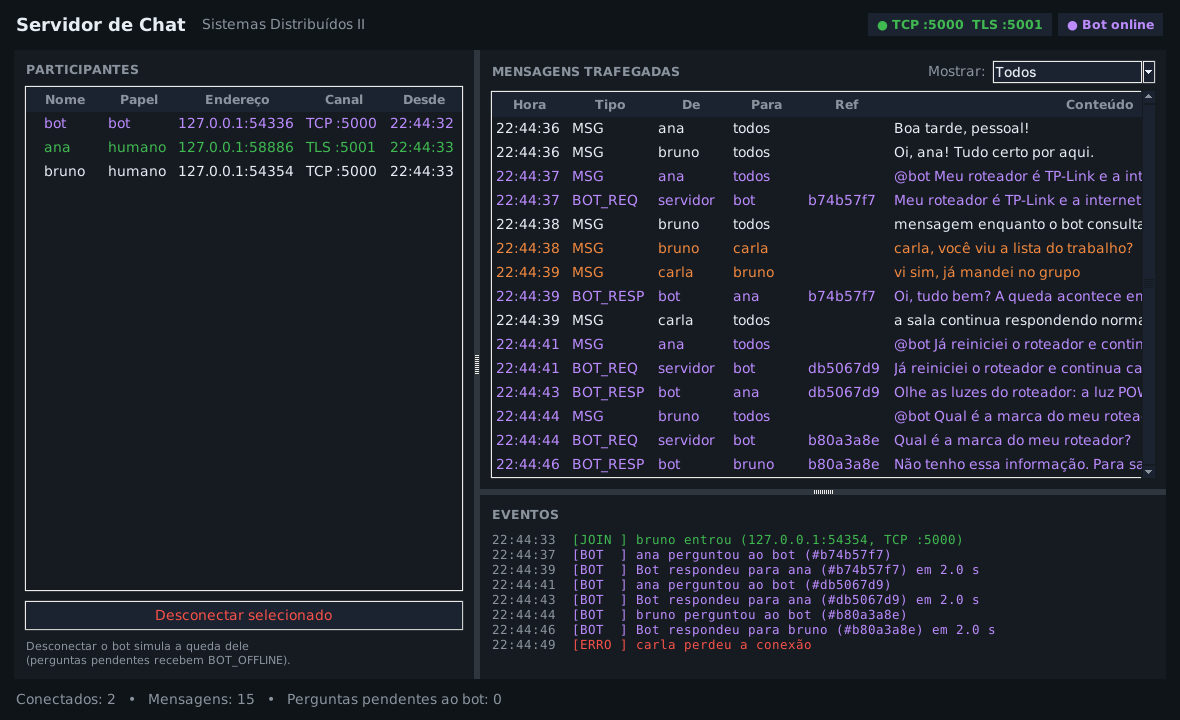
\includegraphics[width=\linewidth]{gui_servidor.png}
\caption{Interface do servidor após uma sessão com ana (TLS), bruno e carla (TCP) e o bot: perguntas
e respostas do bot com o mesmo \cod{ref}, mensagens privadas entre bruno e carla durante a consulta e,
no fim, a queda abrupta da carla (evento em vermelho). Captura gerada em ambiente de teste, com a LLM
substituída por um servidor local que devolve as respostas registradas no cenário real.}
\label{fig:gui-servidor}
\end{figure}

\subsection{Cliente}
O cliente começa numa tela de conexão (nome, servidor, porta e a opção ``Usar TLS'', que troca a porta
para 5001). Depois de conectado (Figura~\ref{fig:gui-clientes}), o selo no canto superior mostra o canal
e, no TLS, a versão e a cifra negociadas. A lista à direita mostra quem está online; clicar num nome
abre a conversa privada. O botão \cod{@bot} prefixa a pergunta. Cada pergunta e cada resposta do bot
aparecem com o identificador curto da solicitação (por exemplo \cod{\#b74b57}).

\begin{figure}[H]
\centering
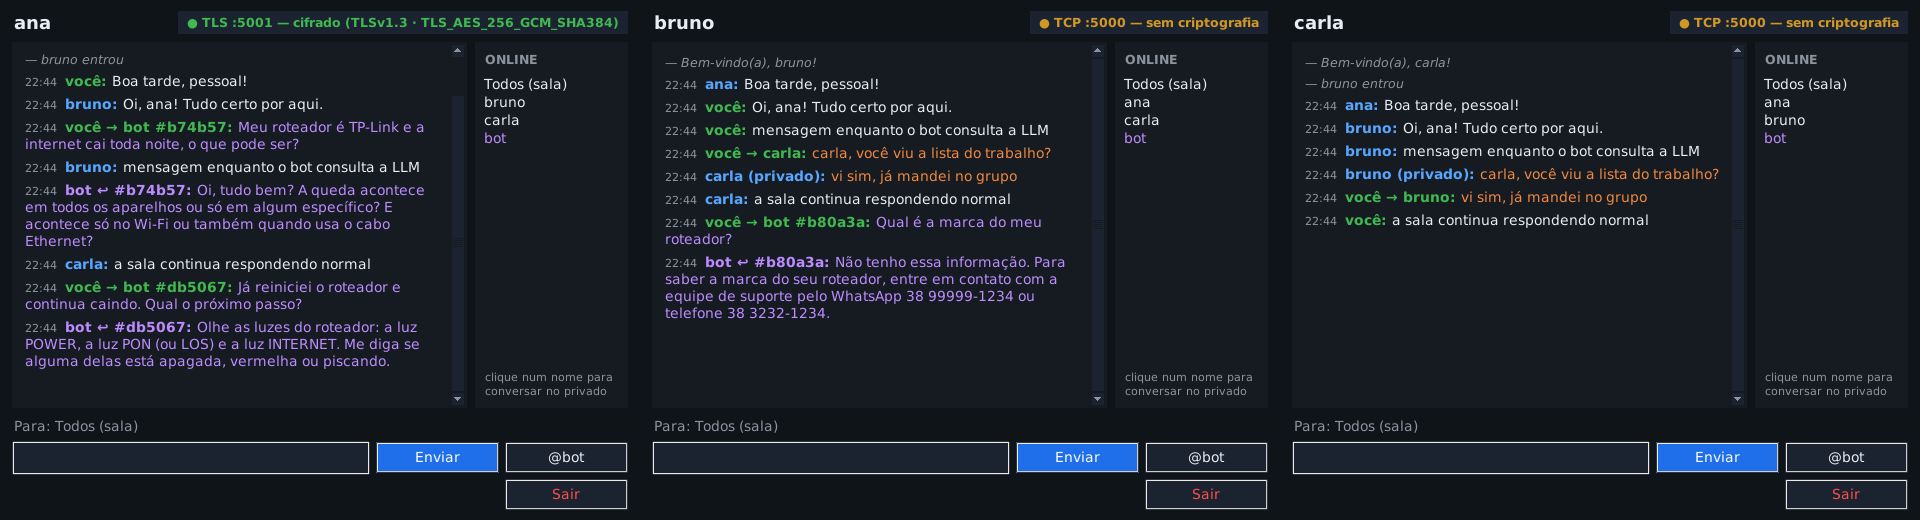
\includegraphics[width=\linewidth]{gui_clientes.png}
\caption{Clientes ana (TLS), bruno e carla (TCP) na mesma sessão da Figura~\ref{fig:gui-servidor}.
Cada usuário vê só as respostas do bot às próprias perguntas.}
\label{fig:gui-clientes}
\end{figure}

% ================================================================== 7
\section{Criptografia das mensagens}\label{sec:cripto}

\subsection{Mecanismo}
Foi usado \textbf{TLS sobre os próprios sockets}, com o módulo \cod{ssl} da biblioteca padrão. O
servidor abre uma segunda porta (5001) com exatamente o mesmo protocolo de aplicação: o socket
aceito é envolvido por \cod{SSLContext.wrap\_socket} dentro da thread do cliente, e daí em diante o
código de leitura e escrita é o mesmo da porta 5000. Os clientes e o bot escolhem o canal com a opção
``Usar TLS'' (ou \cod{--tls}).

Na demonstração a sessão negociada é \textbf{TLS~1.3 com \cod{TLS\_AES\_256\_GCM\_SHA384}}:
\begin{itemize}
  \item a troca de chaves é ECDHE: cada sessão gera chaves novas, que não dependem da chave privada do
        servidor (sigilo futuro);
  \item a chave privada do certificado (ECDSA P-256) só assina o \emph{handshake}, provando que o
        servidor é o dono do certificado;
  \item os dados vão cifrados com AES-256 em modo GCM, criptografia autenticada: além de esconder o
        conteúdo, qualquer alteração dos bytes no caminho é detectada e a conexão é encerrada.
\end{itemize}

\subsection{Certificados}
O script \cod{certs/gerar\_certificados.py} cria uma \textbf{autoridade certificadora de teste} e um
\textbf{certificado do servidor} assinado por ela:
\begin{center}
\small
\begin{tabularx}{\linewidth}{l X}
\toprule
\textbf{Arquivo} & \textbf{Conteúdo} \\
\midrule
\cod{ca.crt}       & CA de teste (ECDSA P-256, \cod{BasicConstraints CA:TRUE}, \cod{keyCertSign}). É o único
                     arquivo que os clientes precisam ter: é a âncora de confiança. \\
\cod{ca.key}       & Chave da CA; usada só para assinar o certificado do servidor. \\
\cod{servidor.crt} & Certificado do servidor: ECDSA P-256, SAN \cod{DNS:localhost} e \cod{IP:127.0.0.1},
                     \cod{extendedKeyUsage serverAuth}, validade de 365 dias. \\
\cod{servidor.key} & Chave privada do servidor (fica só no servidor). \\
\bottomrule
\end{tabularx}
\end{center}
As chaves (\cod{*.key}) e os certificados gerados estão no \cod{.gitignore}: cada máquina gera os seus
com \cod{python certs/gerar\_certificados.py}. O script usa o pacote \cod{cryptography} e, na falta
dele, o OpenSSL instalado.

\subsection{Validação feita pelo cliente}
O contexto do cliente (\cod{common/tls.py}) valida o servidor explicitamente:
\begin{lstlisting}[style=py]
ctx = ssl.create_default_context(ssl.Purpose.SERVER_AUTH, cafile="certs/ca.crt")
ctx.verify_mode = ssl.CERT_REQUIRED          # certificado obrigatório, cadeia até a nossa CA
ctx.check_hostname = True                    # 127.0.0.1 precisa estar no SAN
ctx.minimum_version = ssl.TLSVersion.TLSv1_2
ctx.verify_flags |= ssl.VERIFY_X509_STRICT   # regras da RFC 5280
\end{lstlisting}
O cliente confia apenas na CA de teste (\cod{cafile}), e não nas autoridades do sistema operacional.
Se o certificado não vier dessa CA, ou não valer para o endereço usado, a conexão é recusada antes
de qualquer mensagem do chat.

\textbf{Teste negativo.} Com o servidor iniciado com \cod{--certificado-falso} (certificado de outra
CA, gerado por \cod{gerar\_certificados.py --falsos}), o cliente recusa a conexão
(Figura~\ref{fig:recusado}). Os testes automáticos também cobrem certificado de outra CA e
certificado com nome errado.

\begin{figure}[H]
\centering
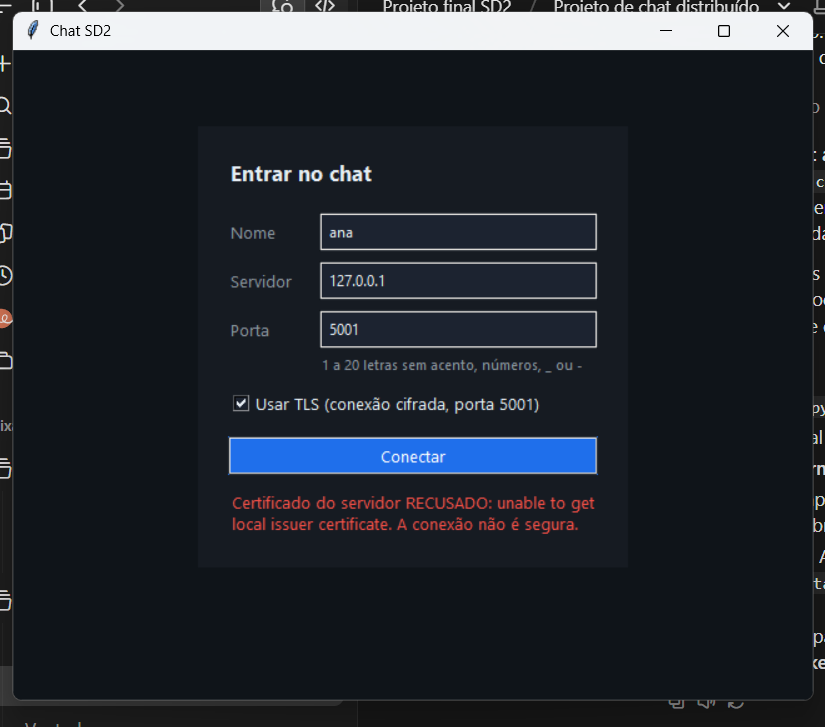
\includegraphics[width=0.55\linewidth]{tls_certificado_recusado.png}
\caption{Cliente recusando um servidor com certificado de outra autoridade.}
\label{fig:recusado}
\end{figure}

\subsection{Enlaces protegidos e onde ocorre a decifragem}\label{sec:enlaces}
O TLS protege \textbf{cada enlace cliente--servidor}, não a mensagem de ponta a ponta:
\begin{enumerate}
  \item a ana cifra a mensagem no \cod{wrap\_socket} do cliente;
  \item os bytes trafegam cifrados até a porta 5001;
  \item o servidor \textbf{decifra} a mensagem no \cod{wrap\_socket} da thread que atende a ana;
        dentro do processo do servidor ela está em claro, porque ele precisa ler o envelope para
        rotear;
  \item no repasse, a mensagem é cifrada de novo, com as chaves da sessão de cada destinatário que
        esteja na porta 5001; para quem está na porta 5000, ela segue em claro.
\end{enumerate}

\begin{center}
\small
\begin{tabularx}{\linewidth}{l l X}
\toprule
\textbf{Enlace (demonstração)} & \textbf{Canal} & \textbf{Proteção} \\
\midrule
ana $\leftrightarrow$ servidor   & TLS :5001 & cifrado e autenticado; decifrado no servidor \\
bruno $\leftrightarrow$ servidor & TCP :5000 & em claro (execução de referência) \\
carla $\leftrightarrow$ servidor & TCP :5000 & em claro (execução de referência) \\
bot $\leftrightarrow$ servidor   & TCP :5000 & em claro (pode usar TLS com \cod{--tls}) \\
bot $\to$ Groq                   & HTTPS     & TLS validado pelas autoridades do sistema \\
\bottomrule
\end{tabularx}
\end{center}
Com \cod{python iniciar.py --tls}, todos os clientes e o bot usam a porta 5001 e nenhum enlace do
chat fica em claro.

\subsection{Análise no Wireshark}\label{sec:wireshark}
As capturas foram feitas no adaptador de \emph{loopback} (Npcap), já que todos os processos estão
no mesmo computador. Uma mensagem conhecida, \cod{SEGREDO-SD2-roteador-TP-Link}, foi enviada nas
duas situações. Filtros usados: \cod{tcp.port == 5000}, \cod{tcp.port == 5001} e
\cod{frame contains "SEGREDO-SD2"}.

\subsubsection*{Execução de referência e execução mista}
Na primeira captura, ana estava na porta 5001 (porta local 58899) e bruno (58900) e carla (58898) na
5000. bruno e depois ana enviaram a mensagem conhecida para a sala. A busca pelo texto
(Figura~\ref{fig:busca}) encontra 4 pacotes, \textbf{todos na porta 5000}:
\begin{center}
\small
\begin{tabular}{l l l}
\toprule
\textbf{Quadro} & \textbf{Fluxo} & \textbf{Conteúdo} \\
\midrule
1126 & bruno (58900) $\to$ servidor & mensagem do bruno, em claro \\
1128 & servidor $\to$ carla (58898) & repasse da mensagem do bruno \\
1204 & servidor $\to$ carla (58898) & repasse da mensagem da \textbf{ana} \\
1206 & servidor $\to$ bruno (58900) & repasse da mensagem da \textbf{ana} \\
\bottomrule
\end{tabular}
\end{center}

\begin{figure}[H]
\centering
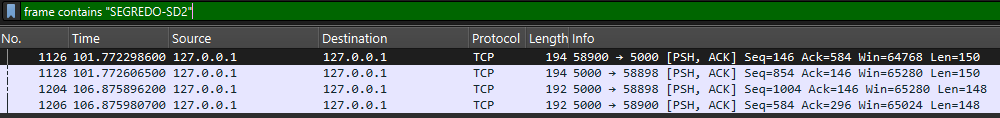
\includegraphics[width=\linewidth]{recorte_busca_segredo.png}
\caption{Busca pela mensagem conhecida: só aparecem pacotes da porta 5000.}
\label{fig:busca}
\end{figure}

``Seguir fluxo TCP'' no fluxo da carla (Figura~\ref{fig:fluxo5000}) mostra o protocolo inteiro em
claro: \cod{HELLO}, \cod{WELCOME}, \cod{USERS}, \cod{JOIN} e as duas mensagens, com remetente e
conteúdo legíveis. Qualquer um com acesso à rede veria a conversa.

\begin{figure}[H]
\centering
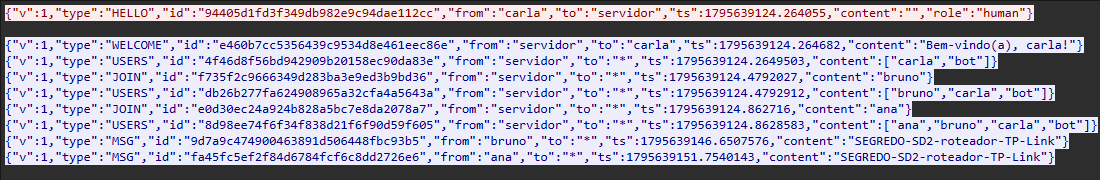
\includegraphics[width=\linewidth]{recorte_5000_fluxo_tcp.png}
\caption{Fluxo TCP da carla na porta 5000: todas as mensagens legíveis, inclusive a enviada pela ana.}
\label{fig:fluxo5000}
\end{figure}

O mesmo intervalo na porta 5001 (Figura~\ref{fig:tls5001}) só tem registros \emph{TLSv1.3
Application Data}. A mensagem da ana para o servidor é o quadro 1202, e o repasse da mensagem do bruno
para a ana é o quadro 1130. Nenhum dos dois é encontrado pela busca, porque o texto só existe cifrado.

\begin{figure}[H]
\centering
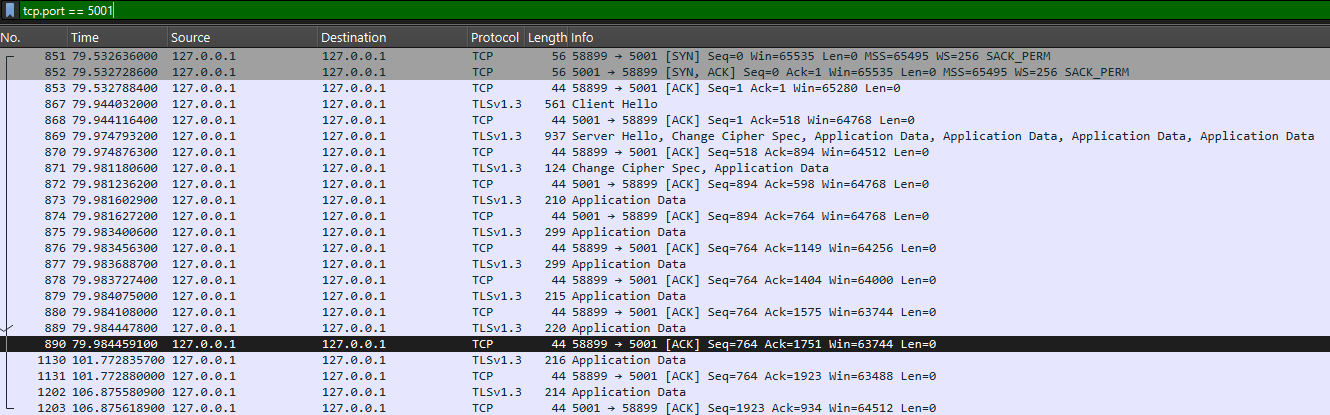
\includegraphics[width=\linewidth]{recorte_5001_tls.png}
\caption{Conexão da ana na porta 5001: \emph{handshake} TLS~1.3 e, depois, apenas \emph{Application Data}.}
\label{fig:tls5001}
\end{figure}

Três observações sobre a captura:
\begin{itemize}
  \item \textbf{\emph{Handshake}.} Depois do \emph{Client Hello} (quadro 867), o servidor responde com
        \emph{Server Hello} e \emph{Application Data}. No TLS~1.3, o certificado e a confirmação do
        \emph{handshake} já viajam cifrados. Em seguida, o registro de 210 bytes enviado pela ana é o
        \cod{HELLO} do chat; os dois de 299 bytes vindos do servidor são os \emph{tickets} de sessão do
        TLS~1.3; e os seguintes são o \cod{WELCOME} e o \cod{USERS}, todos cifrados.
  \item \textbf{Tamanho.} A mesma mensagem ocupa 150 bytes de dados TCP em claro (quadro 1126) e 172
        bytes no TLS (quadro 1130). A diferença de 22 bytes é o cabeçalho do registro TLS (5), o tipo de
        conteúdo interno (1) e a etiqueta de autenticação do GCM (16). O TLS esconde o conteúdo, mas
        não o tamanho aproximado nem o momento do envio.
  \item \textbf{Enlace, não ponta a ponta.} A mensagem que a ana enviou cifrada (quadro 1202)
        aparece \emph{em claro} nos quadros 1204 e 1206, no repasse para carla e bruno, que estavam na
        porta 5000. Isso confirma o comportamento descrito na Seção~\ref{sec:enlaces}: o servidor
        decifra para rotear, e cada enlace só fica protegido se usar TLS.
\end{itemize}

\subsubsection*{Execução com todos os enlaces em TLS}
Na segunda captura, todos os clientes e o bot usaram a porta 5001 (\cod{iniciar.py --tls}). As três
conexões aparecem com \emph{handshake} completo e só \emph{Application Data}
(Figura~\ref{fig:todostls}); os três primeiros quadros (RST) são tentativas de uma execução anterior.
Com a mensagem conhecida enviada de novo, a busca pelo texto \textbf{não encontra nenhum dos 285
pacotes} (Figura~\ref{fig:buscavazia}), enquanto a mensagem aparece normalmente na tela da ana
(Figura~\ref{fig:anatls}).

\begin{figure}[H]
\centering
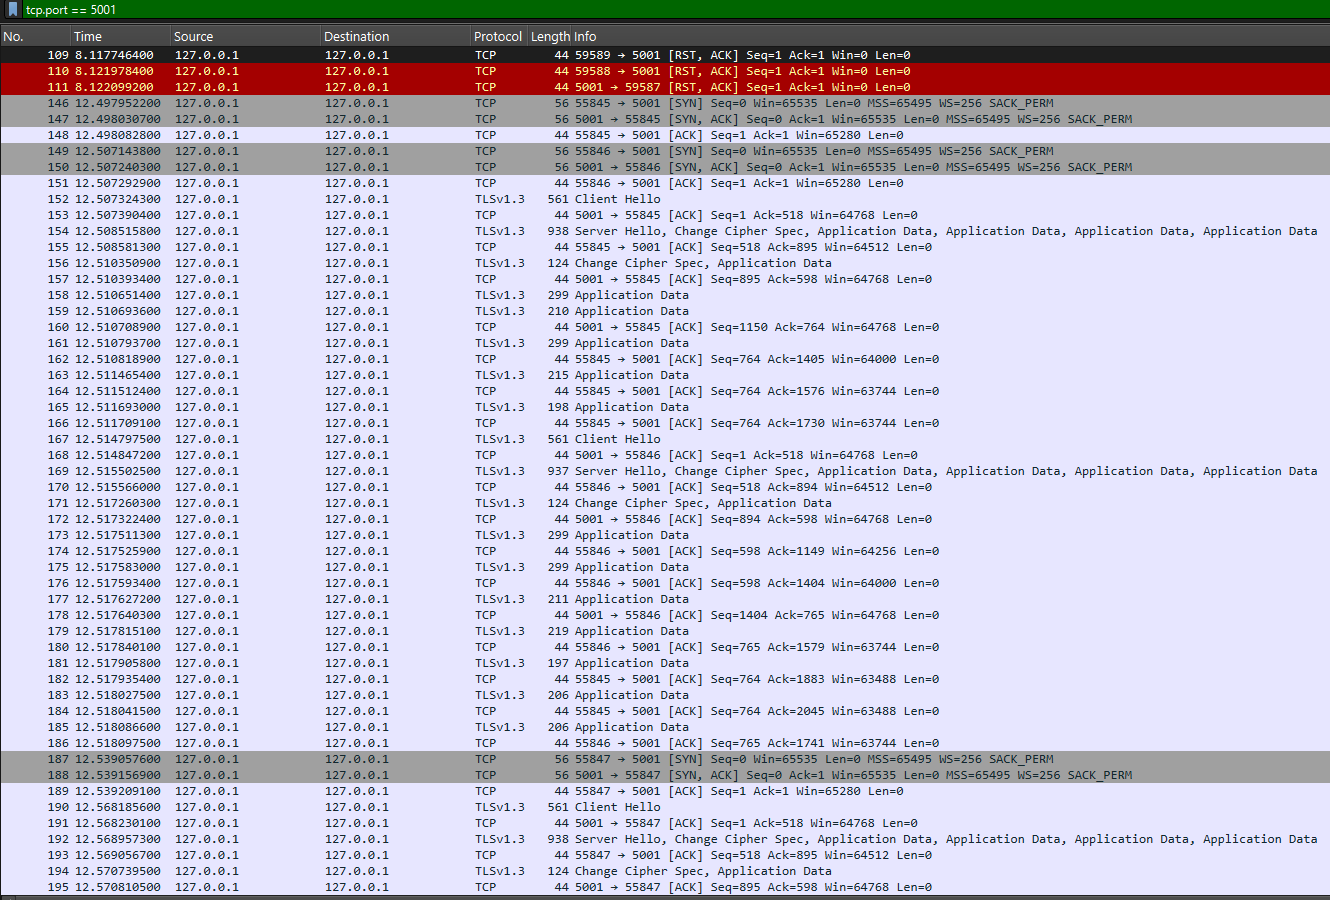
\includegraphics[width=\linewidth]{recorte_todos_tls.png}
\caption{Todos os clientes na porta 5001: três \emph{handshakes} TLS~1.3 e apenas dados cifrados.}
\label{fig:todostls}
\end{figure}

\begin{figure}[H]
\centering
\begin{minipage}[b]{0.56\linewidth}
  \centering
  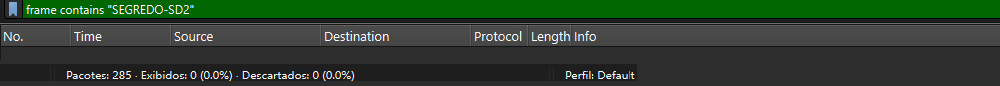
\includegraphics[width=\linewidth]{recorte_busca_vazia.png}
  \caption{Busca pela mensagem com todos em TLS: nenhum resultado (``Exibidos: 0'') entre os 285 pacotes.}
  \label{fig:buscavazia}
\end{minipage}\hfill
\begin{minipage}[b]{0.4\linewidth}
  \centering
  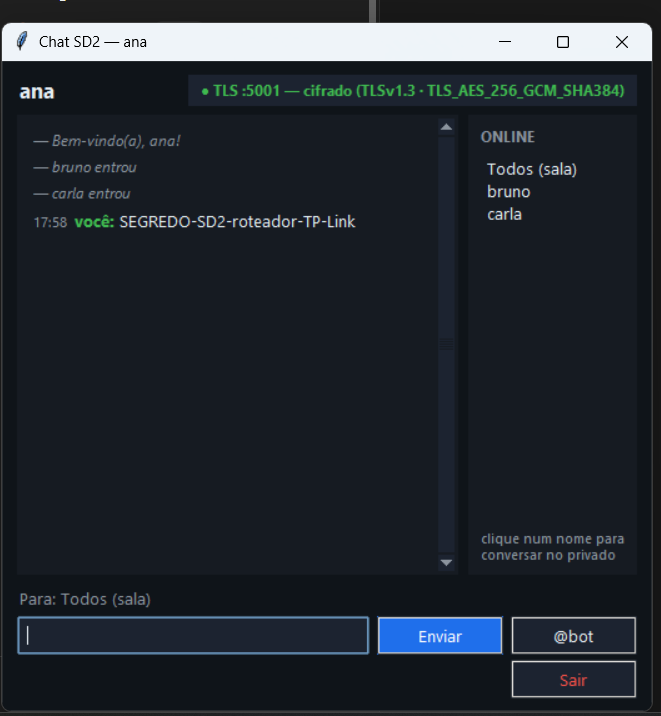
\includegraphics[width=\linewidth]{cliente_ana_tls_mensagem_enviada.png}
  \caption{A mesma mensagem na tela da ana (TLS~1.3).}
  \label{fig:anatls}
\end{minipage}
\end{figure}

\textbf{Por que o conteúdo fica protegido.} No \emph{handshake}, cliente e servidor combinam por ECDHE
uma chave de sessão que nunca trafega pela rede. O cliente aceita a sessão só depois de verificar que o
certificado vem da nossa CA e vale para \cod{127.0.0.1}, então não há como um intermediário se colocar no
meio sem ser recusado. A partir daí cada registro é cifrado com AES-256-GCM. Quem captura os pacotes vê
apenas bytes indistinguíveis de aleatórios e, sem a chave da sessão, não consegue recuperar o texto nem
alterá-lo sem ser detectado.

% ================================================================== 8
\section{Bot com modelo de linguagem}\label{sec:bot}

\subsection{Modelo e forma de execução}
\begin{center}
\small
\begin{tabularx}{\linewidth}{l X}
\toprule
\textbf{Item} & \textbf{Valor} \\
\midrule
Serviço        & API do Groq, compatível com o formato da OpenAI
                 (\cod{https://api.groq.com/openai/v1/chat/completions}) \\
Modelo         & \cod{openai/gpt-oss-120b} (configurável por \cod{LLM\_MODEL} no \cod{.env}) \\
Parâmetros     & \cod{max\_tokens = 700}; \cod{reasoning\_effort = low} (respostas mais rápidas e menos
                 tokens gastos com o raciocínio) \\
Chamada        & \cod{urllib.request} (biblioteca padrão), HTTPS, chave no cabeçalho
                 \cod{Authorization}; tempo limite de 15~s \\
Execução       & processo separado: \cod{python -m bot} (ou \cod{--tls}); conecta-se ao servidor como
                 cliente com \cod{role:"bot"} \\
Credencial     & lida do \cod{.env} (fora do repositório); o repositório traz só o \cod{.env.example} \\
\bottomrule
\end{tabularx}
\end{center}
A chamada HTTPS à LLM é só um complemento do bot: toda a troca de mensagens do chat, inclusive
perguntas e respostas, passa pelos sockets do servidor.

\subsection{Acionamento e correlação}
O bot é acionado pela menção \cod{@bot} no início da mensagem. O servidor transforma a mensagem num
\cod{BOT\_REQ}, que leva o \cod{ref} (o \cod{id} da mensagem original) e o usuário em
\cod{on\_behalf\_of}. O bot responde com \cod{from:"bot"}, \cod{to} igual ao usuário e o mesmo
\cod{ref}. O servidor confere os dois campos contra a tabela de pendentes antes de repassar
(Seção~\ref{sec:protocolo}), e o cliente usa o \cod{ref} para mostrar a qual pergunta a resposta
pertence. Uma resposta com \cod{ref} desconhecido, já expirado ou para outro usuário é descartada e
registrada como evento.

\subsection{Instrução de comportamento}
O tema é o atendimento técnico de um provedor de internet por fibra. A instrução de sistema foi
adaptada de um material preparado pela Bruna para o provedor fictício \emph{Virtual Net}. O original
tinha cerca de 9 mil \emph{tokens}, mais do que o limite de 8 mil \emph{tokens} por minuto do plano
gratuito do Groq para esse modelo; uma única pergunta já seria recusada. Por isso ele foi condensado
para cerca de 1,5 mil \emph{tokens} (\cod{bot/prompts/instrucao.md}), mantendo:
\begin{itemize}
  \item a identidade: assistente virtual, sem acesso ao sistema da empresa, que nunca diz ter feito
        algo nele;
  \item as regras: não inventar valores ou políticas; texto simples e curto (até 5 frases); uma
        etapa por vez; nunca orientar mexer na fibra (só olhar); nunca usar o botão \emph{reset}; não
        pedir dados pessoais; recusar assuntos fora do provedor;
  \item os dados da empresa: horários, canais, pagamentos, desbloqueio, vencimentos, planos e
        preços, fidelidade e instalação; o roteiro de suporte técnico; quando indicar a equipe; e
        como tratar o cancelamento.
\end{itemize}
A \textbf{base de luzes do roteador} (\cod{base\_luzes.md}) só é anexada quando a pergunta ou as últimas
mensagens do usuário falam de luzes, roteador, fibra ou falta de conexão, o que economiza
\emph{tokens} nas demais perguntas. A data e a hora atuais também entram na instrução, para o bot
dizer se a equipe está atendendo naquele momento. Como o modelo às vezes usa \emph{markdown} mesmo
instruído a não usar, o bot remove negrito, títulos e marcadores antes de enviar a resposta, já que o
chat mostra texto puro. Os arquivos originais estão preservados em \cod{bot/prompts/original/}.

\subsection{Histórico por usuário}\label{sec:historico}
\begin{itemize}
  \item \textbf{Limite adotado: as 4 últimas trocas (pergunta + resposta) de cada usuário}, ou seja,
        até 8 mensagens, além da instrução de sistema (\cod{HISTORICO\_TROCAS=4}).
  \item Cada usuário tem a sua \cod{deque(maxlen=8)}, indexada pelo nome em minúsculas. Quando passa
        do limite, a troca mais antiga sai sozinha. O usuário só vê o próprio contexto.
  \item No histórico fica só o começo de cada resposta (600 caracteres); o usuário sempre recebe a
        resposta inteira. Isso mantém o contexto e reduz os \emph{tokens} de cada chamada.
  \item A troca só é registrada depois de uma resposta bem-sucedida; uma falha não polui o histórico.
  \item O histórico fica em memória, protegido por lock, e é perdido quando o bot é reiniciado.
\end{itemize}

\subsection{Tratamento de falhas da LLM}\label{sec:falhasllm}
\begin{center}
\small
\begin{tabularx}{\linewidth}{l l X}
\toprule
\textbf{Situação} & \textbf{Código} & \textbf{Comportamento} \\
\midrule
Sem resposta em 15~s     & \cod{LLM\_TIMEOUT}     & \cod{BOT\_ERR} ao usuário; o chat segue normal \\
HTTP 429 (limite de uso) & \cod{LLM\_RATE\_LIMIT} & se o \cod{Retry-After} for de até 8~s, espera e tenta mais uma vez;
                                                     senão avisa na hora \\
HTTP 401/403             & \cod{LLM\_AUTH}        & chave inválida ou ausente \\
HTTP 404, sem rede, resposta vazia & \cod{LLM\_UNAVAILABLE} & mensagem com o motivo \\
Erro inesperado no bot   & \cod{LLM\_UNAVAILABLE} & o pedido falha, mas o bot continua atendendo \\
\bottomrule
\end{tabularx}
\end{center}
Para a demonstração, \cod{python -m bot --simular-falha timeout} reduz o tempo limite para 0,01~s
(e \cod{--simular-falha chave} usa uma chave inválida), de modo que a chamada ao Groq falha de verdade.

\subsection{Exemplos de respostas reais}
Testes com o Groq em 25/11/2026 (\cod{python -m bot.llm "pergunta"}):
\begin{center}
\small
\begin{tabularx}{\linewidth}{>{\raggedright\arraybackslash}p{4.2cm} X}
\toprule
\textbf{Pergunta} & \textbf{Resposta (resumida)} \\
\midrule
``oi'' & ``Oi, aqui é o assistente virtual da Virtual Net. Como posso ajudar?'' \\
``quais os planos de vocês?'' & Os 4 planos com os preços corretos, fidelidade de 12 meses, consulta ao
SPC, instalação em até 7 dias úteis, equipamentos em comodato. \\
``estou sem internet, a luz LOS está vermelha piscando'' & Olhar o cabo da fibra \emph{sem tocar};
reiniciar (30~s na tomada); se continuar, procurar o suporte pelo WhatsApp ou telefone. \\
``posso apertar o botão reset do roteador?'' & ``Não. Não recomendo usar o botão reset.'' e explica o
reinício pela tomada (com ONU: ligar a ONU primeiro). \\
``me passa uma receita de bolo'' & ``Desculpe, só consigo ajudar com assuntos da Virtual Net.'' \\
\bottomrule
\end{tabularx}
\end{center}

% ================================================================== 9
\section{Testes e evidências}\label{sec:testes}

\subsection{Testes automáticos}
São 105 testes com \cod{unittest}, que sobem o servidor real em portas livres e, no lugar do Groq,
usam uma API HTTP local no mesmo formato (os testes não dependem de internet nem gastam cota).
\begin{center}
\small
\begin{tabularx}{\linewidth}{>{\ttfamily}l r X}
\toprule
{\normalfont\bfseries Arquivo} & \textbf{Testes} & \textbf{O que cobre} \\
\midrule
test\_protocolo.py & 22 & Delimitação (mensagem partida, várias num \cod{recv}, UTF-8 cortado), limites, nomes, \cod{@bot} \\
test\_servidor.py  & 35 & \emph{Handshake}, nomes, entrada/saída/queda, expulsão, 30 clientes simultâneos,
                         sala/privado, percurso do \cod{@bot}, conversa durante a consulta, tempo limite, queda do bot \\
test\_cliente.py   & 11 & Rede do cliente contra o servidor real: envio sem bloquear durante a consulta, \cod{ref}, saída e queda \\
test\_bot\_rede.py & 7  & \cod{ref} e usuário corretos, consultas em paralelo, falha da LLM vira \cod{BOT\_ERR} \\
test\_bot\_llm.py  & 21 & Chamada à LLM (401/404/429, tempo limite, sem rede), histórico, instrução e orçamento de \emph{tokens} \\
test\_tls.py       & 9  & TLS junto com TCP, bot por TLS, recusa de outra CA e de nome errado, bytes legíveis só na 5000 \\
\bottomrule
\end{tabularx}
\end{center}

\subsection{Cenário real com os componentes separados}
O script \cod{validar.py} verifica o ambiente e os certificados, roda os testes e executa um cenário em
processos separados: servidor, bot com o Groq de verdade, ana por TLS e bruno e carla por TCP. Resultado
da execução de 25/11/2026 às 19:33 (Windows 11, Python 3.14):
\begin{center}
\small
\begin{tabularx}{\linewidth}{X c}
\toprule
\textbf{Verificação} & \textbf{Resultado} \\
\midrule
ana conectada por TLS :5001 (TLSv1.3, \cod{TLS\_AES\_256\_GCM\_SHA384}); bruno e carla por TCP & OK \\
5 mensagens bruno $\to$ carla entregues \emph{durante} a consulta à LLM (média de 3~ms) & OK \\
Bot respondeu à ana em 1,0~s com o mesmo \cod{ref} & OK \\
Pergunta de continuação respondida considerando a anterior & OK \\
Contextos separados: o bot não sabe a marca do roteador da ana quando o bruno pergunta & OK \\
Respostas do bot entregues só a quem perguntou & OK \\
Falha da LLM vira \cod{BOT\_ERR LLM\_TIMEOUT} e o sistema continua & OK \\
Chat funcionando depois da falha & OK \\
Saída normal avisada (\cod{LEFT}) e queda abrupta detectada (\cod{CONNECTION\_LOST}) & OK \\
\bottomrule
\end{tabularx}
\end{center}

\textbf{Continuação e contextos separados.} A ana disse que o roteador é TP-Link e a internet cai toda
noite; o bot perguntou se a queda acontece em todos os aparelhos. Na continuação (``Já reiniciei o roteador
e continua caindo''), o bot seguiu o roteiro e pediu para olhar as luzes do roteador. Logo depois, o bruno
perguntou ``Qual é a marca do meu roteador?'', e o bot respondeu que não tinha essa informação: o contexto da
ana não vazou para ele.

\subsection{Arquivos de evidência}
Na pasta \cod{evidencias/} do repositório:
\begin{itemize}
  \item \cod{validacao\_<data>.txt}: resumo da validação;
  \item \cod{concorrencia\_<data>.txt}: linha do tempo do cenário real;
  \item \cod{servidor\_<data>.log}: registro do servidor no cenário real;
  \item capturas do Wireshark (Figuras~\ref{fig:busca} a \ref{fig:buscavazia}) e do teste negativo do certificado.
\end{itemize}

% ================================================================== 10
\section{Limitações encontradas}\label{sec:limitacoes}
\begin{itemize}
  \item \textbf{Proteção por enlace, não ponta a ponta.} O servidor vê as mensagens em claro, e um
        destinatário na porta 5000 recebe em claro uma mensagem enviada por TLS. Criptografia ponta a
        ponta exigiria troca de chaves entre os usuários e impediria o servidor de rotear pelo conteúdo
        (o \cod{@bot}).
  \item \textbf{Metadados visíveis.} Mesmo no TLS, a captura mostra portas, tamanhos aproximados e
        horários das mensagens.
  \item \textbf{CA de teste.} A autoridade é criada pelo próprio grupo e precisa ser distribuída aos
        clientes. Não há revogação de certificados nem autenticação dos clientes pelo servidor: qualquer
        um que alcance a porta pode entrar com um nome livre, sem senha.
  \item \textbf{Limites do plano gratuito do Groq.} Com 8 mil \emph{tokens} por minuto, perguntas
        disparadas em sequência rápida chegam a receber \cod{LLM\_RATE\_LIMIT}; isso motivou a
        condensação da instrução, a reserva de 700 \emph{tokens} para a resposta e a nova tentativa
        automática. O serviço também depende de internet.
  \item \textbf{Respostas da LLM.} Apesar das regras da instrução, o modelo pode errar ou simplificar uma
        orientação. Por isso a instrução manda indicar a equipe sempre que a informação não estiver no texto.
  \item \textbf{Estado só em memória.} Histórico do bot, mensagens e participantes não são persistidos;
        reiniciar o bot apaga os contextos.
  \item \textbf{Ponto único de falha.} Todo o tráfego passa por um servidor; se ele cair, o chat para. Há
        um único bot, e não existe ordem global entre mensagens de conexões diferentes (só dentro de cada
        conexão).
  \item \textbf{Uma thread por conexão.} O modelo é simples e adequado à escala do trabalho (testado com
        30 clientes), mas para milhares de conexões seria melhor E/S assíncrona (\cod{selectors} ou
        \cod{asyncio}).
  \item \textbf{Ambiente.} A demonstração roda em um único computador (\emph{loopback}). Em rede, bastaria
        ajustar o endereço e gerar o certificado com o IP do servidor no SAN.
\end{itemize}

% ================================================================== 11
\section{Conclusão}
O trabalho resultou num chat em que servidor, clientes e bot são processos independentes que se
comunicam apenas por sockets TCP, com um protocolo documentado que resolve a delimitação das mensagens, a
identificação do remetente e a correlação entre pergunta e resposta. O uso de uma thread por conexão,
combinado com locks de escopo curto e com filas entre a rede e as interfaces, permitiu que a conversa entre
os usuários continuasse enquanto o bot consultava a LLM, como mostram os testes e o cenário real. O canal
TLS validou o servidor pela autoridade de teste e, nas capturas do Wireshark, tornou ilegível a mensagem
conhecida, que na porta sem criptografia aparecia por inteiro. As capturas também deixaram claro o limite do
mecanismo: a proteção vale por enlace. O bot gerou respostas reais e coerentes com as regras do provedor
fictício, mantendo contextos separados por usuário e tratando as falhas da LLM sem afetar o restante do chat.

\appendix
% ================================================================== A
\section{Instalação, configuração e execução}
Requisitos: Python 3.10 ou superior com Tkinter (já incluído no instalador do Windows).
\begin{lstlisting}
git clone https://github.com/PedroSarmentoo/ProjetoFinalSD2
cd ProjetoFinalSD2
copy .env.example .env               # e coloque a chave do Groq em LLM_API_KEY
pip install cryptography             # só para gerar os certificados
python certs/gerar_certificados.py   # CA de teste + certificado do servidor

python iniciar.py                    # servidor (GUI) + bot + ana, bruno e carla
python iniciar.py --tls-para ana     # só a ana por TLS (comparação dos canais)
python iniciar.py --tls              # todos os clientes e o bot por TLS
python -m bot --simular-falha timeout   # bot com falha da LLM (demonstração)

python validar.py                    # ambiente, certificados, testes e cenário real
python -m unittest discover -s tests # só os testes automáticos
\end{lstlisting}
Cada componente também pode ser iniciado em seu próprio terminal: \cod{python -m servidor},
\cod{python -m bot} e \cod{python -m cliente ana --conectar}.

% ================================================================== B
\section{Exemplo completo de troca de mensagens}
\begin{lstlisting}
ana  → servidor {"v":1,"type":"HELLO","id":"a1…","from":"ana","to":"servidor","ts":…,"content":"","role":"human"}
servidor → ana  {"v":1,"type":"WELCOME","id":"s1…","from":"servidor","to":"ana","ts":…,"content":"Bem-vindo(a), ana!"}
servidor → ana  {"v":1,"type":"USERS","id":"s2…","from":"servidor","to":"*","ts":…,"content":["ana","bot","bruno"]}

ana  → servidor {"v":1,"type":"MSG","id":"m42","from":"ana","to":"*","ts":…,"content":"@bot minha internet cai toda noite"}
servidor → bot  {"v":1,"type":"BOT_REQ","id":"s9","from":"servidor","to":"bot","ts":…,"ref":"m42",
                 "on_behalf_of":"ana","content":"minha internet cai toda noite"}
bot → servidor  {"v":1,"type":"BOT_RESP","id":"b7","from":"bot","to":"ana","ts":…,"ref":"m42","content":"A queda …"}
servidor → ana  {"v":1,"type":"BOT_RESP","id":"b7","from":"bot","to":"ana","ts":…,"ref":"m42","content":"A queda …"}

bot → servidor → ana {"v":1,"type":"BOT_ERR","id":"b8","from":"bot","to":"ana","ts":…,"ref":"m43",
                      "code":"LLM_TIMEOUT","content":"A LLM não respondeu em 15 s. Tente novamente."}
\end{lstlisting}

\end{document}
